\documentclass[12pt,a4paper]{article}

\usepackage[a4paper,
            mag=1000, includefoot,
            left=3cm, right=1.5cm, top=2cm, bottom=2cm, headsep=1cm, footskip=1cm]{geometry}
\usepackage[T2A]{fontenc}
\usepackage[utf8]{inputenc}
\usepackage[english,russian]{babel}
\usepackage{xcolor}
\usepackage{amsmath,amssymb,amsfonts,dsfont}
\usepackage{algorithmic}
\usepackage{graphicx,wrapfig}

\newcommand{\todo}[1]{ {\color{red} TODO: {#1}}}
\newcommand{\figref}[1]{(Рис. \ref{#1})}
\renewcommand{\it}[1]{{\textit{#1}}}

\begin{document}
\title{Деревья решений. Ансамбли деревьев решений: бэггинг, случайный лес}
\author{А. Рукавишникова, М. Сандул, В. Страшко}
\maketitle

Как и прежде, мы будем рассматривать задачу обучения с учителем (supervised learning). Пусть есть некоторая модель данных:
\begin{equation*}
\eta = f(\xi, \Theta) + \epsilon,
\end{equation*}
где $\epsilon$ --- некоторый шум, $f$ --- неизвестная с точностью до параметров $\Theta$ функция, $\xi = (\xi_1, \ldots, \xi_p)$ --- случайный вектор, $\eta$ --- зависимая случайная величина. Пусть у нас есть $n$ реализаций случайных величин $\eta$ и $\xi$:
\begin{equation*}
Y = (y_1, \ldots, y_n)^\intercal,\\
\mathbb X =  
\begin{pmatrix} 
x_{1, 1} & x_{1, 2} & \ldots & x_{1, p} \\
x_{2, 1} & x_{2, 2} & \ldots & x_{2, p} \\
\vdots & \vdots & \ldots & \vdots\\
x_{n, 1} & x_{n, 2} & \ldots & x_{n, p},
\end{pmatrix} 
\end{equation*}
где $Y$ --- реализации $\eta$, $\mathbb X$ --- реализации $\xi$, в которой столбцы соответствуют реализациям случайных величин $\xi_i$, а строки --- номеру реализации. Обозначим $x_i$ --- i-ю строку матрицы $\mathbb X$. По набору этих реализации мы хотим найти оценку $\hat\Theta$ неизвестных параметров $\Theta$. Один из наиболее часто используемых критериев для построения оценки $\Theta$ --- это метод наименьших квадратов:

\begin{equation*}
\hat\Theta = \arg \min_{\tilde\Theta} \sum_{i=1}^{n}{(y_i - f(x_i. \tilde\Theta))^2}.
\end{equation*} 

\section{Кусочно-постоянные функции}

Пусть есть некоторое множество $\Omega$ и его разбиение $\mathcal A = \{A_i\}_{i=1}^{\infty}$,  $\Omega = \vee_{i=1}^{\infty}{A_i}$. Разбиение может быть конечным, тогда часть $A_i = \emptyset$. Кусочно-постоянной функцией, заданной на разбиении $\mathcal A$ назовем функцию $f: \Omega \rightarrow \mathbb R$, определенную следующим образом: \
\begin{equation*}
f(x) = \sum_{i=1}^{\infty}{c_i \cdot \mathds{1}_{A_i}(x)},
\end{equation*}
где $\mathds{1}_{A_i}(x)$ --- индикаторная функция множества $A_i$, $c_i \in \mathbb R, |c_i| < \infty$. Поскольку, $A_i$ --- разбиение множества $\Omega$ (то есть $\forall i \neq j: A_i \cap A_j = \emptyset$), то в любой точке $x \in \Omega$  $f$ принимает одно из значений $c_i$.\par

Не умаляя общности, мы будем считать считать, что $\Omega \subseteq \mathbb R^p$. Кусочно-постоянные функции --- это очень удобный инструмент для аппроксимации функций. С помощью кусочно-постоянных функций возможно с произвольной точность аппроксимировать любую $g: \mathbb R^p \rightarrow \mathbb R$, такую что $|g| < \infty$ и у функции не более чем счетное количество разрывов. Такое свойство следует из того, что множество кусочно-постоянных функций всюду плотно на множестве таких функций $g$ (факт из функционального анализа). Кусочно-постоянные функции используется, например, для аппроксимации значений определенных интегралов ---  метод прямоугольников.\par

Произвольное разбиение $\mathcal A$ не очень удобный объект для представления. Мы рассмотрим случай, когда каждое из множеств $A_i$ --- это многомерный прямоугольник. Такие множества удобно представлять в виде набора неравенств для каждой координаты: $x \in A_i \iff a_{i,1} \leq x_1 < b_{i, 1}, \ldots, a_{i,p} \leq x_p < b_{i,p}$, где $x_i$ --- i-я координата вектора $x$. $f$ мы можем переписать в следующем виде \eqref{eq:parconst}:

\begin{equation}
f(x) = 
\begin{cases}
c_1 & \mbox{if }  a_{1,1} \leq x_1 < b_{1, 1}, \ldots, a_{1,p} \leq x_p < b_{1,p} \\
c_2 & \mbox{if }  a_{2,1} \leq x_1 < b_{2, 1}, \ldots, a_{2,p} \leq x_p < b_{2,p} \\
\vdots & \vdots \\
c_i & \mbox{if }  a_{i,1} \leq x_1 < b_{i, 1}, \ldots, a_{i,p} \leq x_p < b_{i,p} \\
\vdots & \vdots
\end{cases}
\label{eq:parconst}
\end{equation}

Допустимо, чтобы некоторые неравенства вырождались в равенства. Переход к такому частному случаю имеет смысл потому, что с помощью прямоугольников мы можем аппроксимировать произвольные множества, поэтому аппроксимирующие свойства кусочно-постоянных функций не утрачиваются.\par

Стоит отметить важное свойство кусочно-постоянных функций: множество кусочно-постоянных функций линейно. Это также справедливо и для кусочно-постоянных функций, определенных на разбиениях из прямоугольников.

\section{Деревья решений}

В теории графов дерево --- это связный неориентированный ациклический граф. Другими словами --- это структура состоящая из вершин и ребер, вершины могут быть соединены ребрами. Если граф связный, то из любой вершины мы можем попасть по ребрам в любую. Если граф ациклический, то, выйдя из любой вершины, мы можем вернуться в неё только по тем ребрам, по которым мы из неё вышли.\par

\begin{figure}[h]
\centering
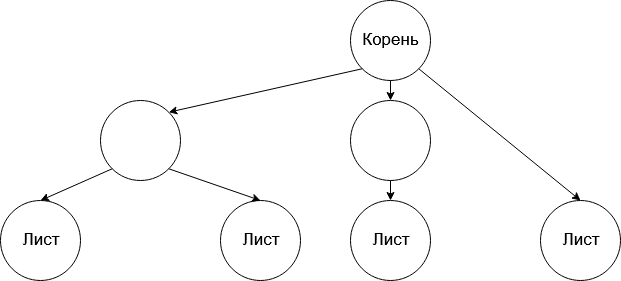
\includegraphics[width=0.6\textwidth]{../resources/simple_tree.png}
\label{fig:simpletree}
\caption{Структура дерева}
\end{figure}

Деревья лежат в основе одноименных структур данных в информатике. У деревьев \figref{fig:simpletree} есть специальные вершины. Одну из вершин мы будем называть корневой, или просто корнем дерева. Любой путь в дереве начинается из этой вершины и направлен от неё. Вершины, в которых заканчивается любой путь, называются листовыми вершинами, или просто листьями. Все остальные вершины называются внутренними. Глубина дерева --- это количество ребер в самом длинном пути от корня к листу.\par

\begin{figure}[h]
\centering
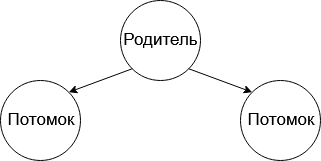
\includegraphics[width=0.33\textwidth]{../resources/parent_child.png}
\label{fig:parentchild}
\caption{Потомки и родители в дереве}
\end{figure}

Вершины, в которые мы можем попасть из текущей, называются потомками. Вершина, из которой мы можем попасть в данную, называется родительской вершиной, или просто родителем \figref{fig:parentchild}. Очевидно, у любой вершины может быть не больше одного родителя, у корня нет родительской вершины. Дерево, у каждой вершины которого не больше двух потомков, называется бинарным.\par

\begin{figure}[h]
\centering
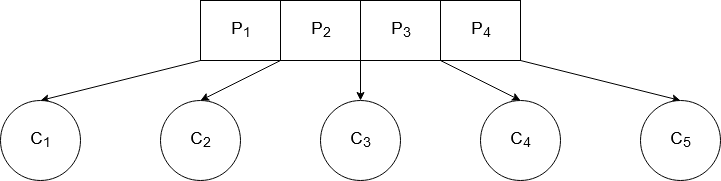
\includegraphics[width=0.6\textwidth]{../resources/decision_tree.png}
\label{fig:dectree}
\caption{Простое не бинарное дерево решений}
\end{figure}

Давайте модифицируем структуру дерева. Пусть у нас есть некоторое множество $\Omega$, и множество предикатов $\mathbb P = \{P_i\}_{i=1}^m$, определенных на $\Omega$. Сопоставим каждой внутренней вершине и корню предикат, а каждой листу число $c_j \in \mathbb R$. Пусть теперь мы хотим сопоставить некоторому объекту $x \in \Omega$ какое-нибудь из чисел, покажем на примере как это сделать. Рассмотрим простое дерево решений глубины 1 \figref{fig:dectree}, это дерево описывает такую функцию \eqref{eq:dectree}:

\begin{equation}
\label{eq:dectree}
f(x) = 
\begin{cases}
c_1 & \mbox{if }  \neg P_1(x) \& \neg P_2(x) \& \neg P_3(x) \& \neg P_4(x) \\
c_2 & \mbox{if }  P_1(x) \& \neg P_2(x) \& \neg P_3(x) \& \neg P_4(x) \\
c_3 & \mbox{if }  \neg P_1(x) \& P_2(x) \& \neg P_3(x) \& \neg P_4(x) \\
c_4 & \mbox{if }  \neg P_1(x) \& \neg P_2(x) \& P_3(x) \& \neg P_4(x) \\
c_5 & \mbox{if }  \neg P_1(x) \& \neg P_2(x) \& \neg P_3(x) \& P_4(x)
\end{cases}
\end{equation}

Теперь нетрудно показать, что любая кусочно-постоянная функция, заданная на прямоугольниках, может быть выражена с помощью дерева решений: произвольные предикаты заменяются на неравенства для значений $x$. На самом деле, достаточно рассматривать бинарные деревья решений, потому что любое не бинарное дерево можно свести к бинарному, нужно просто вынести каждый из предикатов в отдельную вершину.\par

Бинарное дерево очень удобно для построения и определения с помощью языков программирование, поэтому мы будем работать именно с таким представлением кусочно-постоянных функций.

\section{Построение дерева решений}

Итак, вернемся к задаче машинного обучения. Есть обучающая выборка размера $n$: $Y \in \mathbb R ^ n, \mathbb X \in \mathbb R ^ {n \times p}$, $p$ --- количество признаков. Будем считать, что $y_i = f(x_i, \Theta) + \epsilon_i$, где $f$ --- кусочно-постоянная функция, известная с точностью до параметров $\Theta$. Параметры кусочно-постоянной функции --- это, собственно, значения этой функции $\{c_i\}$, а также ограничения на $x$, задающие разбиение исходного множества признаков, числа $\{a_{ij}\}$ и $\{b_{ij}\}$ из определения функции \eqref{eq:parconst}, их предстоит оценить по обучающей выборке.\par

Перебор всех возможных деревьев, которые можно определить на $Y, \mathbb X$, занимает слишком много времени. Можно показать, что это NP-трудная задача, поэтому используется приближенный жадный алгоритм.\par

Вспомним, что кусочно-постоянные функции определены на разбиении исходного множества, и дерево решений, на самом деле, задаёт это разбиение. Значения $c_i$ в листах деревьев на самом деле определяются значениями $y_i$, для которых выполняются все условия во внутренних вершинах и корне, ведущих к этим листьям. Также каждая внутренняя вершина разбивает выборку на две не пересекающиеся части. Итак, алгоритм построения будет заключаться в том, чтобы на текущем шаге один из листов превратить во внутреннюю вершину. Опишем этот алгоритм более подробно.\par

Во-первых, нужен критерий качества разбиения. Если $Y$ --- непрерывная величина, то есть мы решаем задачу регрессии, то в качестве критерия можно выбрать дисперсию внутри элемента разбиения: если при разделении текущей вершины на два листа мы смогли уменьшить дисперсию, значит разбиение хорошее. Чем больше разница между исходной дисперсией в вершине и суммарной дисперсией в новых листьях, тем лучше разбиение.\par

Во-вторых, нужно как выбирать разбиение. Предлагается рассматривать разные варианты условий для каждого признака отдельно.

\section{Объединение деревьев в ансамбль}

Одно решающее дерево довольно слабая модель: часто она даёт относительно невысокое качество предсказания, даже по сравнению с линейными моделями. Усложнение, например увеличение глубины дерева, быстро приводит к переобучению. Возникает идея объединить несколько моделей в одну. 

\subsection{Бэггинг}

Общая схема объединения моделей. Построим $k$ бустрап выборок  $(Y^i, \mathbb X^i)$ из исходной. Для каждой бустрап выборки $(Y^i, \mathbb X^i)$  обучим модель $f_i$. Результирующую модель мы получим по формуле: $f = \frac{1}{k}\sum_{i=1}^{k}{f_i}$.  

\subsection{Случайный лес}

На самом деле, чем меньше корреляция между моделями в ансамбле, тем лучше. Для деревьев возможно уменьшить коэффициент корреляции между функциями путем сэмплирования и признаков на каждом из разбиений: на каждом шаге мы будем выбирать не из всех возможных признаков, а только по некоторому случайному подмножеству.
  
\end{document}